\section{稀疏矩阵计算}
我们的下一个并行模式是稀疏矩阵计算。 在稀疏矩阵中,大多数元素为零。 
存储和处理这些零元素在内存容量、内存带宽、时间和能量方面都是浪费的。 许多重要的现实问题都涉及稀疏矩阵计算。 
由于这些问题的重要性,几种稀疏矩阵存储格式及其相应的处理方法被提出并在该领域得到广泛应用。 
所有这些方法都采用某种类型的压缩技术来避免存储或处理零元素,但代价是在数据表示中引入某种程度的不规则性。 
不幸的是,这种不规则性可能导致并行计算中内存带宽的利用不足、控制流发散和负载不平衡。 
因此,在压缩和正则化之间取得良好的平衡非常重要。 一些存储格式在高度不规则性的情况下实现了更高水平的压缩。 
其他人实现了更适度的压缩水平,同时保持表示更规则。 
众所周知,使用每种存储格式的并行计算的相对性能在很大程度上取决于稀疏矩阵中非零元素的分布。 
了解稀疏矩阵存储格式及其相应并行算法的大量工作,为并行程序员在解决相关问题时应对压缩和正则化挑战提供了重要的背景。

\subsection{背景}
\begin{figure}[H]
	\centering
	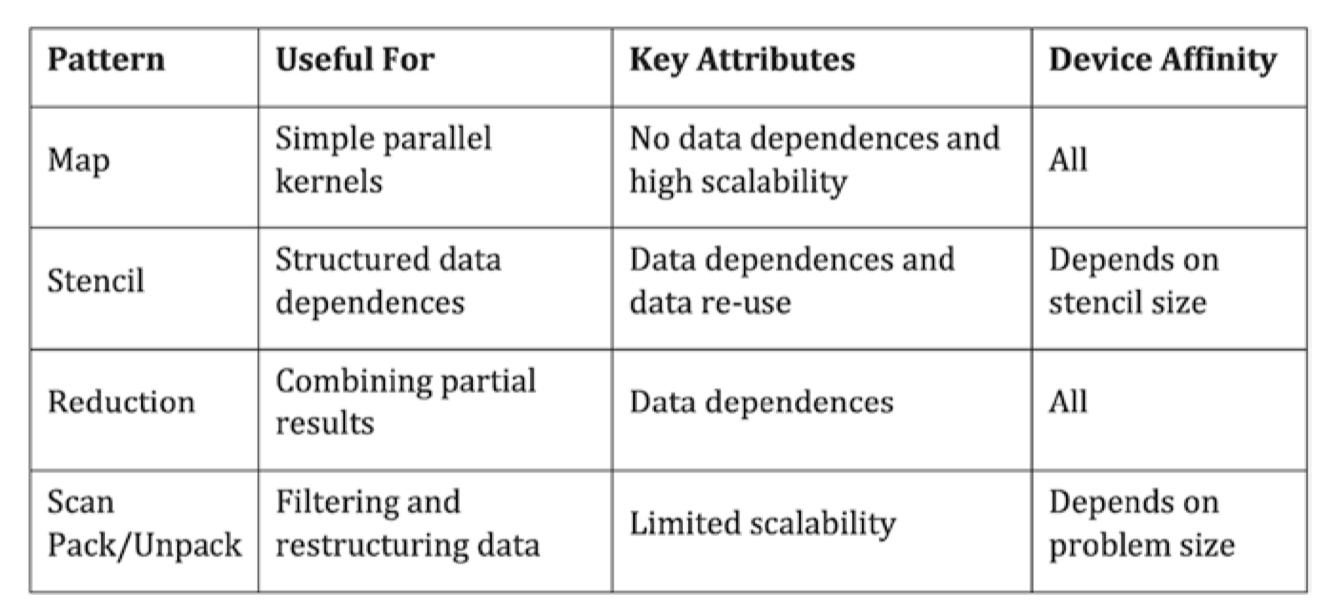
\includegraphics[width=0.9\textwidth]{figs/F14.1.png}
	\caption{\textit{一个简单的稀疏矩阵示例。}}
\end{figure}

稀疏矩阵是大多数元素为零的矩阵。 稀疏矩阵出现在许多科学、工程和金融建模问题中。 例如,矩阵可用于表示线性方程组中的系数。 
矩阵的每一行代表线性系统的一个方程。 在许多科学和工程问题中,所涉及的大量变量和方程都是稀疏耦合的。 
也就是说,每个方程仅涉及少量变量。 
如图 14.1 所示,其中矩阵的每一列对应于一个变量的系数:第 0 列代表 $\mathrm{x}_{0}$,
第 1 列代表 $\mathrm{x}_{1 }$,等等。 
例如,第 0 行在第 0 列和第 1 列中具有非零元素这一事实表明方程 0 中仅涉及变量 $x_{0}$ 和 $x_{1}$ 。 
应该清楚的是,变量 $\mathrm{x}_{0}、\mathrm{x}_{2}$ 和 $\mathrm{x}_{3}$ 出现在方程 1 中,
变量 $\mathrm{x}_{1}$ 和 $\mathrm{x}_{2}$ 在等式 2 中存在,等式 3 中仅存在变量 $x_{3}$ 。 
稀疏矩阵通常以避免存储零元素的格式或表示形式存储。

矩阵通常用于求解 $\mathrm{N}$ 变量的 $\mathrm{N}$ 方程的线性系统,
其形式为 $\mathrm{A}^{*} \mathrm{X}+\mathrm{Y }=0$,其中$\mathrm{A}$是$\mathrm{N} \times \mathrm{N}$矩阵,
$\mathrm{X}$是$\mathrm{N}$变量的向量 ,$\mathrm{Y}$ 是 $\mathrm{N}$ 常量值的向量。 
目标是求解满足所有方程的 $\mathrm{X}$ 变量值。 直观的方法是对矩阵求逆,
使得$\mathrm{X}=\mathrm{A}^{-1} *(-\mathrm{Y})$。 对于中等大小的矩阵,可以通过高斯消除等方法来完成此操作。 
虽然理论上可以使用这些方法来求解稀疏矩阵表示的方程,但许多稀疏矩阵的庞大规模可能会压倒这种直观的方法。 
此外,逆稀疏矩阵通常比原始矩阵大得多,因为逆过程往往会生成许多额外的非零元素,这些元素称为“填充”。 
因此,在解决现实问题时计算和存储逆矩阵通常是不切实际的。

以稀疏矩阵表示的线性方程组可以通过迭代方法更好地求解。 
当稀疏矩阵 $\mathrm{A}$ 为正定时(即,对于所有非零向量 
$\mathrm{x}$,$\mathrm{x}^{\mathrm{T}} \mathrm{Ax}>0$ $\mathrm{R}^{n}$ 中),
可以使用共轭梯度法迭代求解相应的线性系统,并保证收敛到一个解(Hestenes 和 Stiefel,1952)。 
共轭梯度法猜测 X 的解,并执行 A * X + Y,并查看结果是否接近 0 向量。 
如果没有,我们可以使用梯度向量公式来细化猜测的 X,并执行 A * X + Y 的另一次迭代。
这些线性系统的迭代求解方法与我们在第 8 章 Stencil 中介绍的微分方程的迭代求解方法密切相关。

\begin{figure}[H]
	\centering
	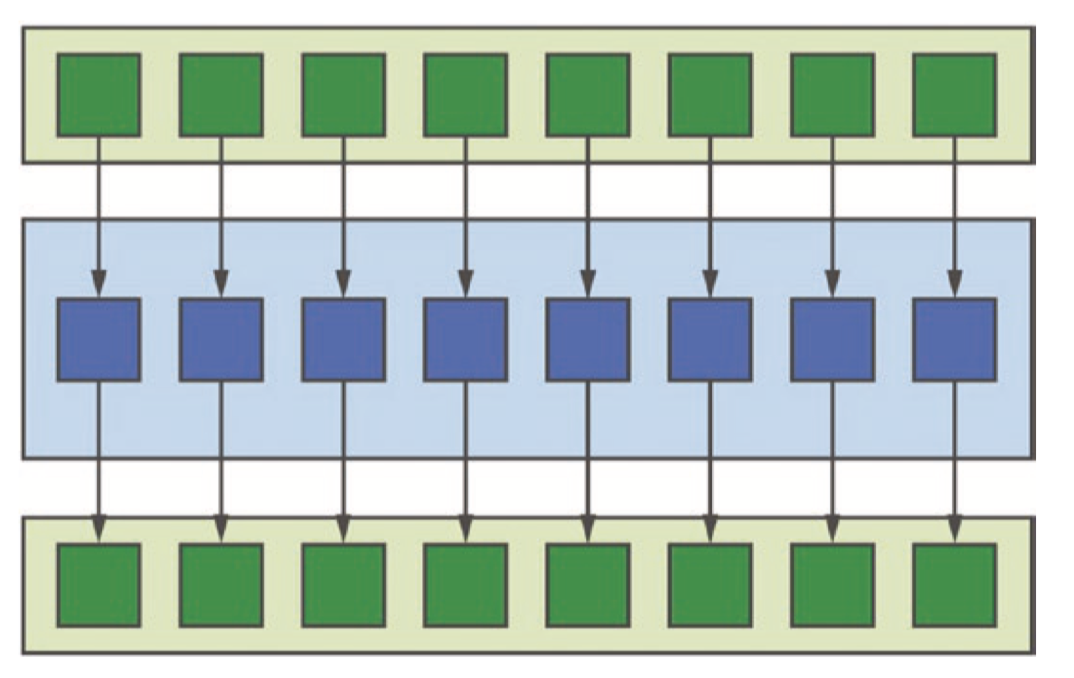
\includegraphics[width=0.9\textwidth]{figs/F14.2.png}
	\caption{\textit{矩阵向量乘法和累加的一个小例子。}}
\end{figure}

求解线性方程组的迭代方法中最耗时的部分是评估 $\mathrm{A}^{*} \mathrm{X}+\mathrm{Y}$,它是稀疏矩阵向量乘法和 积累。 
图 14.2 显示了矩阵向量乘法和累加的一个小例子,其中 A 是稀疏矩阵。 
$\mathrm{A}$ 中的黑色方块代表非零元素。 相反,$\mathrm{X}$ 和 $\mathrm{Y}$ 都是典型的稠密向量。 
也就是说,$\mathrm{X}$ 和 $\mathrm{Y}$ 的大部分元素都持有非零值。 
由于其重要性,已经创建了标准化库函数接口来执行该操作,名称为 SpMV(稀疏矩阵向量乘法和累加)。 
我们将使用 SpMV 来说明并行稀疏矩阵计算中不同存储格式之间的重要权衡。

不同稀疏矩阵存储格式的主要目标是从矩阵表示中删除所有零元素。 
删除所有零元素不仅可以节省存储空间,而且还不需要从内存中取出这些零元素并用它们执行无用的乘法或加法运算。 
这可以显着减少内存带宽和计算资源的消耗。

稀疏矩阵存储格式的结构有多种设计考虑因素。 以下是一些关键考虑因素的列表:
\begin{itemize}
   \item 空间效率(或压缩):使用存储格式表示矩阵所需的内存容量

   \item 灵活性:存储格式使得通过添加或删除非零值来修改矩阵变得容易的程度

   \item 可访问性:存储格式使其易于访问的数据类型

   \item 内存访问效率:存储格式为特定计算启用高效内存访问模式的程度(正则化的一个方面)

   \item 负载平衡:存储格式平衡特定计算的不同线程之间的负载的程度(正则化的另一个方面)

\end{itemize}

在本章中,我们将介绍不同的存储格式,并研究这些存储格式在每个设计考虑因素中的比较。

\subsection{具有 COO 格式的简单 SpMV 内核}
\begin{figure}[H]
	\centering
	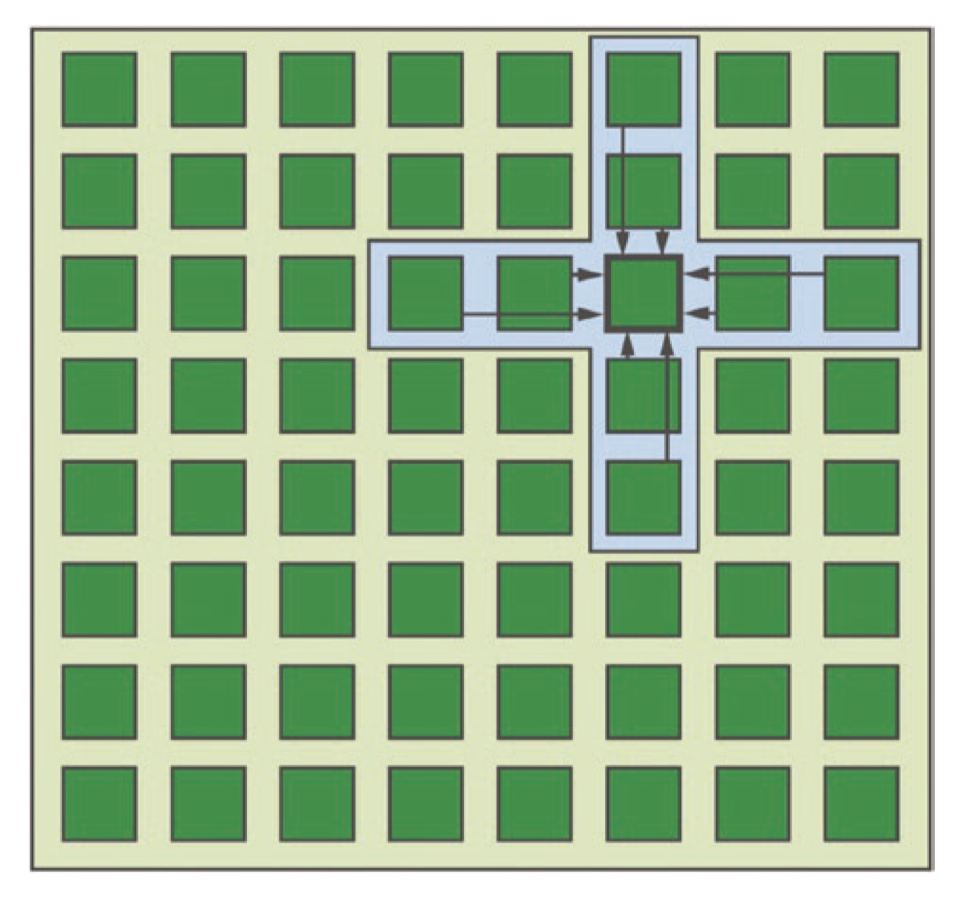
\includegraphics[width=0.9\textwidth]{figs/F14.3.png}
	\caption{\textit{坐标列表 (COO) 格式的示例。}}
\end{figure}

我们将讨论的第一个稀疏矩阵存储格式是坐标列表(COO)格式。 COO 格式如图 14.3 所示。 
COO 将非零值存储在一维数组中,显示为值数组。 每个非零元素都与其列索引和行索引一起存储。 
我们有 colIdx 和 rowIdx 数组来伴随值数组。 
 及其列索引(colIdx[0] 中的 0)和 其行索引(rowldx[0] 中的 0)存储在其他数组中的相同位置。

COO 从存储中完全删除所有零元素。 它确实通过引入 colIdx 和 rowIdx 数组而产生存储开销。 
在我们的小例子中,零元素的数量并不比非零元素的数量大很多,存储开销实际上比不存储零元素节省的空间还要多。 
然而,应该清楚的是,对于绝大多数元素为零的稀疏矩阵,引入的开销远远小于不存储零所节省的空间。 
例如,在稀疏矩阵中,只有 $1 \%$ 的元素是非零值,COO 表示的总存储(包括所有开销)
将约为存储零和 $3 \%$ 所需的空间 非零元素。

\begin{figure}[H]
	\centering
	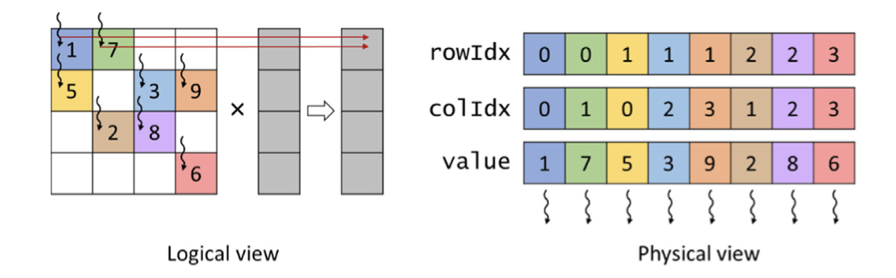
\includegraphics[width=0.9\textwidth]{figs/F14.4.png}
	\caption{\textit{SpMV 与 COO 格式并行化的示例。}}
\end{figure}

\begin{figure}[H]
	\centering
	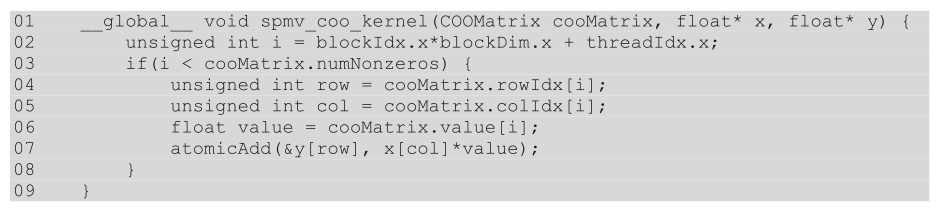
\includegraphics[width=0.9\textwidth]{figs/F14.5.png}
	\caption{\textit{并行 SpMV/COO 内核。}}
\end{figure}

使用以 COO 格式表示的稀疏矩阵并行执行 SpMV 的一种方法是将线程分配给矩阵中的每个非零元素。 
这种并行化方法的示例如图 14.4 所示,相应的代码如图 14.5 所示。 
在此方法中,每个线程标识其负责的非零元素的索引(第 02 行)并确保它在边界内(第 03 行)。 
接下来,线程分别从 rowIdx、colIdx 和 value 数组中识别其负责的非零元素的行索引(第 04 行)、
列索引(第 05 行)和值(第 06 行)。 然后,它在与列索引对应的位置查找输入向量值,将其乘以非零值,
然后将结果累加到相应行索引处的输出值(第 07 行)。 
原子操作用于累加,因为多个线程可能更新相同的输出元素,就像图 14.4 中映射到矩阵第 0 行的前两个线程的情况一样。 
显然,任何 SpMV 计算代码都会反映假定的存储格式。 因此,我们将存储格式添加到内核名称中,以明确所使用的组合。 
我们还将图 14.5 中的 SpMV 代码称为 SpMV/COO。

\begin{figure}[H]
	\centering
	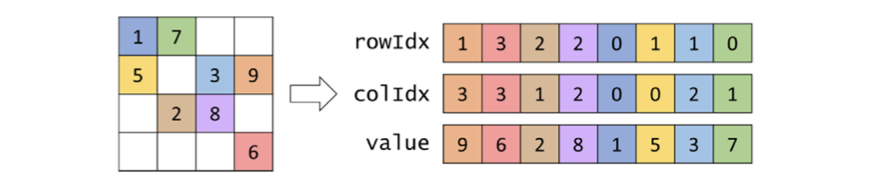
\includegraphics[width=0.9\textwidth]{figs/F14.6.png}
	\caption{\textit{重新排序坐标列表 (COO) 格式。}}
\end{figure}

现在我们根据第 14.1 节中列出的设计考虑因素来检查 $\mathrm{COO}$ 格式:
空间效率、灵活性、可访问性、内存访问效率和负载平衡。 为了空间效率,我们推迟讨论,当我们引入其他格式时。 
为了灵活性,我们观察到,只要我们以相同的方式重新排序 rowIdx、colIdx 和 value 数组,
我们就可以以 $\mathrm{COO}$ 格式任意重新排序元素,而不会丢失任何信息。 
这是通过使用图 14.6 中的小示例来说明的,其中我们对 rowIdx、colIdx 和 value 的元素进行了重新排序。 
现在 value[0] 实际上包含原始稀疏矩阵第 1 行和第 3 列的元素。 
因为我们还随数据值一起移动了行索引和列索引值,所以我们可以正确识别该元素在原始稀疏矩阵中的位置。

在 COO 格式中,我们可以按照我们想要的任何顺序处理元素。 
rowIdx[i] 标识的正确 y 元素将从 value[i] 和 x[colIdx[i]] 的乘积中获得正确的贡献。 
如果我们确保以某种方式对所有值元素执行此操作,则无论我们处理这些元素的顺序如何,我们都将计算出正确的最终答案。

读者可能会问为什么我们要对这些元素重新排序。 一个原因是数据可能是从不按特定顺序提供非零值的文件中读取的,
并且我们仍然需要一种一致的方式来表示数据。 因此,在最初构造矩阵时,$\mathrm{COO}$ 是一种流行的存储格式选择。 
另一个原因是,不必提供任何排序,只需在三个数组的末尾添加条目即可将非零添加到矩阵中。 
因此,当在整个计算过程中修改矩阵时,$\mathrm{COO}$ 是一种流行的存储格式选择。 
我们将在第 14.5 节中看到 COO 格式灵活性的另一个好处。

我们要考虑的下一个设计考虑因素是可访问性。 对于给定的非零值,COO 可以轻松访问其相应的行索引和列索引。 
$\mathrm{COO}$ 的这一特性可以实现 SpMV/COO 中非零元素的并行化。 
另一方面,对于给定的行或列,COO 并不容易访问该行或列中的所有非零值。 
因此,如果计算需要按行或按列遍历矩阵,则 $\mathrm{COO}$ 不是一个好的格式选择。

对于内存访问效率,我们参考图 14.4 中的物理视图来了解线程如何从内存访问矩阵数据。 
访问模式是这样的:连续的线程访问形成 COO 格式的三个数组中的每一个中的连续元素。 因此 SpMV/COO 对矩阵的访问是合并的。

对于负载平衡,我们记得每个线程负责一个非零值。 
因此,所有线程都负责相同的工作量,这意味着除了边界处的线程之外,我们不希望 SpMV/COO 中发生任何控制分歧。

SpMV/COO 的主要缺点是需要使用原子操作。 使用原子操作的原因是多个线程被分配给同一行中的非零值,因此需要更新相同的输出值。 
如果同一行中的所有非零值都分配给同一线程,使得该线程将是唯一更新相应输出值的线程,则可以避免原子操作。 
但是,请记住 $\mathrm{COO}$ 格式不提供这种可访问性。 
在 $\mathrm{COO}$ 格式中,对于给定行,访问该行中的所有非零值并不容易。 
在下一节中,我们将看到另一种提供这种可访问性的存储格式。

\subsection{使用 CSR 格式对行非零值进行分组}
在上一节中,我们看到使用 COO 格式并行化 SpMV 会受到原子操作使用的影响,因为相同的输出值由多个线程更新。 
如果同一线程负责一行的所有非零值,则可以避免这些原子操作,这需要存储格式使我们能够访问给定行中该行中的所有非零值。 
这种可访问性是由压缩稀疏行 (CSR) 存储格式提供的。

\begin{figure}[H]
	\centering
	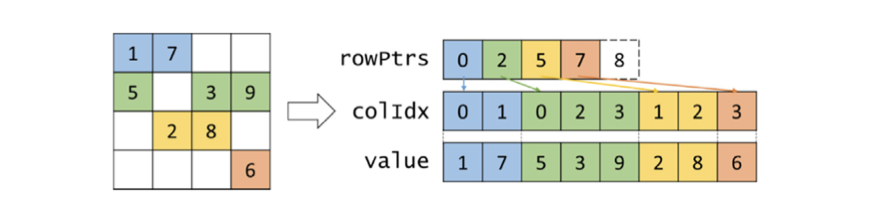
\includegraphics[width=0.9\textwidth]{figs/F14.7.png}
	\caption{\textit{压缩稀疏行 (CSR) 格式的示例。}}
\end{figure}

图14.7说明了如何使用CSR格式存储图14.1中的矩阵。 与 COO 格式一样,CSR 将非零值存储在一维数组中,
如图 14.2 中的值数组所示。 但是,这些非零值按行分组。 例如,我们首先存储第 0 行的非零元素(1 和 7),
然后是第 1 行的非零元素(5、3 和 9),最后是第 2 行的非零元素(2 和 8),然后 最后是第 3 (6) 行的非零元素。

也类似于 $\mathrm{COO}$ 格式,CSR 将值数组中的每个非零元素存储在 colIdx 数组中相同位置的列索引。 
当然,这些列索引按值按行分组。 在图 14.7 中,每行的非零值按其列索引以升序排列。 
以这种方式对非零值进行排序会产生有利的内存访问模式,但这不是必需的。 
每行中的非零值不一定按其列索引排序,并且本节中介绍的内核仍然可以正常工作。 
当每行中的非零值按其列索引排序时,CSR 的值数组(和 colIdx 数组)的布局可以视为消除所有零元素后矩阵的行优先布局。

COO 格式和 CSR 格式之间的主要区别在于,CSR 格式将 rowIdx 数组替换为 rowPtrs 数组,
该数组存储 colIdx 和 value 数组中每行非零值的起始偏移量。 
在图 14.7 中,我们展示了一个 rowPtrs 数组,其元素是每行起始位置的索引。 
即,rowPtrs[0] 表示第 0 行从值数组的位置 0 开始,rowPtrs[1] 表示第 1 行从位置 2 开始,依此类推。 
请注意,rowPtrs [4] 存储不存在的“第 4 行”的起始位置。 
这是为了方便,因为某些算法需要使用下一行的起始位置来描绘当前行的结尾。 
这个额外的标记提供了一种方便的方法来定位第 3 行的结束位置。

\begin{figure}[H]
	\centering
	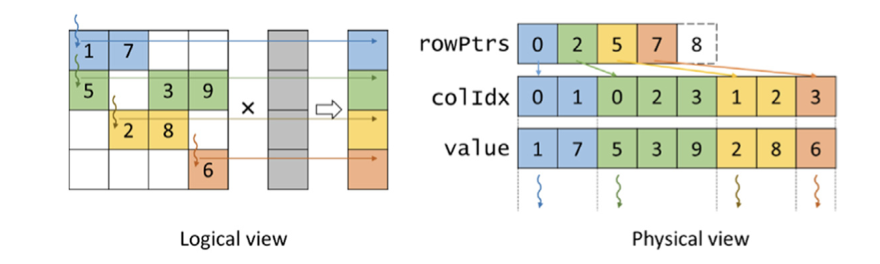
\includegraphics[width=0.9\textwidth]{figs/F14.8.png}
	\caption{\textit{SpMV 与 CSR 格式并行化的示例。}}
\end{figure}

要使用以 CSR 格式表示的稀疏矩阵并行执行 SpMV,可以为矩阵的每一行分配一个线程。 
这种并行化方法的示例如图 14.8 所示,相应的代码如图 14.9 所示。 
在这种方法中,每个线程都会识别它负责的行(第 02 行)并确保它在边界内(第 03 行)。 
接下来,线程循环遍历其行的非零元素以执行点积(第 05-06 行)。 
为了查找该行的非零元素,线程在 rowPtrs 数组 (rowPtrs[row]) 中查找它们的起始索引。 
它还通过查找下一行的非零值的起始索引 (rowPtrs [row +1] ) 来找到它们的结束位置。 
对于每个非零元素,线程标识其列索引(第 07 行)和值(第 08 行)。 
然后,它在与列索引对应的位置查找输入值,将其乘以非零值,并将结果累加到局部变量 sum(第 09 行)。 
sum 变量在点积循环开始之前初始化为 0(第 04 行),并在循环结束后累加到输出向量(第 11 行)。 
请注意,将总和累加到输出向量不需要原子操作。 
原因是每一行都由单个线程遍历,因此每个线程将写入不同的输出值,如图 14.8 所示。

并行 SpMV/CSR 内核。 现在我们根据 14.1 节中列出的设计考虑因素来检查 CSR 格式:
空间效率、灵活性、可访问性、内存访问效率和负载平衡。 对于空间效率,我们观察到 CSR 比 COO 的空间效率更高。 
COO 需要三个数组:rowIdx、colIdx 和 value,每个数组的元素数量与非零数的数量一样多。 
相比之下,CSR 仅需要两个数组:colIdx 和 value,其元素数量与非零值的数量一样多。 
第三个数组 rowPtrs 仅需要与行数加一一样多的元素,这使得它比 COO 中的 rowIdx 数组小得多。 
这种差异使得 CSR 比 COO 更节省空间。

就灵活性而言,我们观察到在向矩阵添加非零值时,CSR 的灵活性不如 COO。 
在 $\mathrm{COO}$ 中,只需将非零附加到数组末尾即可添加非零。 在 CSR 中,要添加的非零必须添加到其所属的特定行。 
这意味着后面的行的非零元素都需要移位,并且后面的行的行指针都需要相应地递增。 
因此,将非零添加到 CSR 矩阵比将它们添加到 $\mathrm{COO}$ 矩阵要昂贵得多。

对于可访问性,CSR 可以轻松访问给定行中的非零值。 
CSR 的这一功能支持 SpMV/CSR 中的跨行并行化,这使得它与 SpMV/COO 相比可以避免原子操作。 
在现实世界的稀疏矩阵应用中,通常有数千到数百万行,每行包含数十到数百个非零元素。 
这使得跨行并行化显得非常合适:有很多线程,并且每个线程都有大量的工作。 
另一方面,对于某些应用程序,稀疏矩阵可能没有足够的行来充分利用所有 GPU 线程。 
在此类应用程序中,COO 格式可以提取更多并行性,因为非零数多于行数。 
此外,对于给定列,CSR 并不容易访问该列中的所有非零值。 
因此,如果需要轻松访问列的所有元素,应用程序可能需要维护额外的、更加面向列的矩阵布局。

\begin{figure}[H]
	\centering
	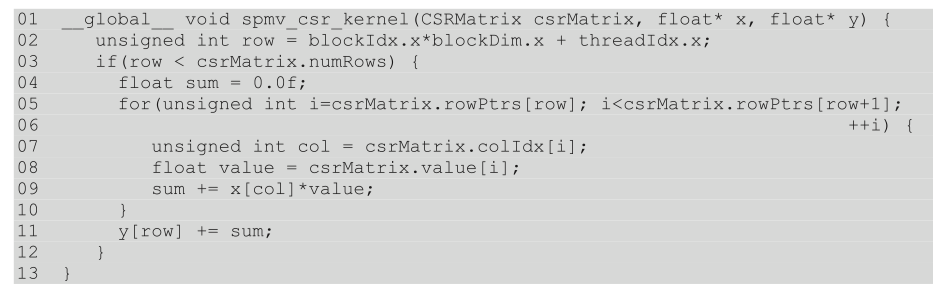
\includegraphics[width=0.9\textwidth]{figs/F14.9.png}
	\caption{\textit{并行 SpMV/CSR 内核。}}
\end{figure}

对于内存访问效率,我们参考图 14.8 中的物理视图,了解线程在点积循环的第一次迭代期间如何从内存访问矩阵数据。 
访问模式使得连续的线程访问相距较远的数据元素。 
特别是,线程 $0、1、2$ 和 3 将在其点积循环的第一次迭代中分别访问 value[0]、value[2]、value[5] 和 value[7]。 
然后,它们将在第二次迭代中分别访问 value[1]、value[3]、value[6] 和无数据,依此类推。 
结果,图 14.9 中并行 SpMV/CSR 内核对矩阵的访问没有合并。 内核没有有效利用内存带宽。

对于负载平衡,我们观察到 SpMV/CSR 内核在所有 warp 中可能存在显着的控制流分歧。 
点积循环中线程所进行的迭代次数取决于分配给该线程的行中非零元素的数量。 由于行间非零元素的分布可以是随机的,因此相邻行可以具有非常不同数量的非零元素。 因此,在大多数甚至所有warp中可能存在广泛的控制流发散。

综上所述,我们已经看到,CSR 相对于 COO 的优点在于它具有更好的空间效率,
并且它使我们能够访问行的所有非零值,从而允许我们通过在 SpMV/CSR 中跨行并行计算来避免原子操作 。 
另一方面,CSR 相对于 COO 的缺点是,它在向稀疏矩阵添加非零元素方面提供的灵活性较差,它表现出不适合合并的内存访问模式,
并且会导致高控制发散。 在以下部分中,我们将讨论与 CSR 相比牺牲一些空间效率的其他存储格式,以改善内存合并并减少控制发散。 
请注意,在 GPU 上从 $\mathrm{COO}$ 转换为 CSR 对于读者来说是一个很好的练习,
使用多个基本并行计算原语,包括直方图和前缀和。

\subsection{使用 ELL 格式改进内存合并}
非合并内存访问的问题可以通过对稀疏矩阵数据应用数据填充和转置来解决。 
这些思想被用在 ELL 存储格式中,其名称来自于 ELLPACK 中的稀疏矩阵包,
ELLPACK 是一个用于解决椭圆边值问题的包(Rice 和 Boisvert,1984)。

\begin{figure}[H]
	\centering
	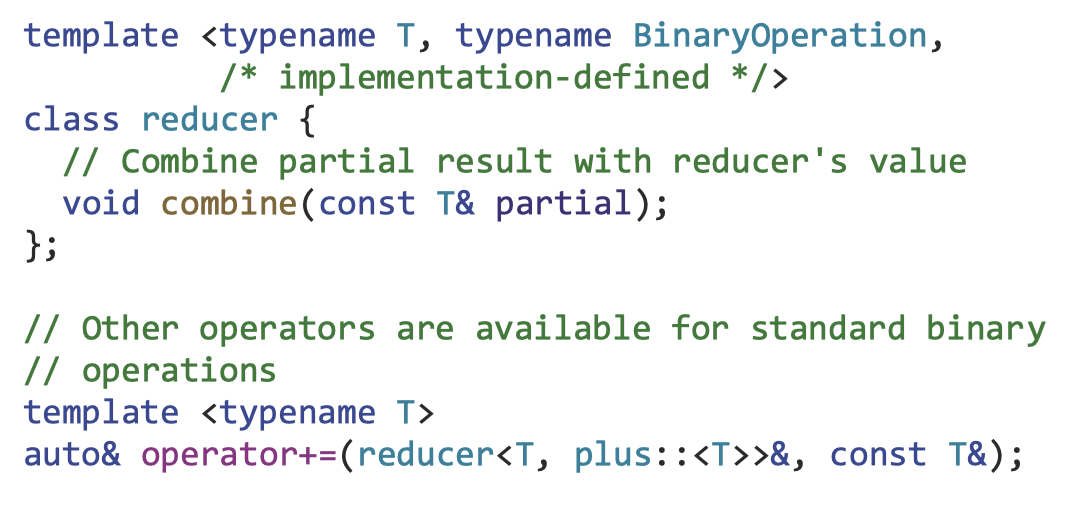
\includegraphics[width=0.9\textwidth]{figs/F14.10.png}
	\caption{\textit{ELL 存储格式示例。}}
\end{figure}

理解 ELL 格式的一个简单方法是从 CSR 格式开始,如图 14.10 所示。 
根据按行对非零元素进行分组的 CSR 表示,我们确定具有最大非零元素数量的行。 
然后,我们将填充元素添加到非零元素之后的所有其他行,以使它们与最大行的长度相同。 这使得矩阵成为矩形矩阵。 
对于我们的小型稀疏矩阵示例,我们确定第 1 行具有最大元素数。 
然后,我们向第 0 行添加一个填充元素,向第 2 行添加一个填充元素,向第 3 行添加两个填充元素,以使它们的长度相同。 
这些附加的填充元素在图 14.11 中显示为带 * 的正方形。 现在矩阵变成了一个矩形矩阵。 
请注意,colIdx 数组也需要以相同的方式进行填充,以保留其与values 数组的对应关系。

\begin{figure}[H]
	\centering
	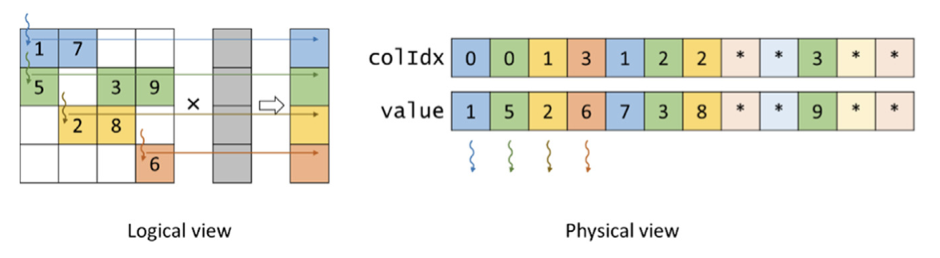
\includegraphics[width=0.9\textwidth]{figs/F14.11.png}
	\caption{\textit{SpMV 与 ELL 格式并行化的示例。}}
\end{figure}

我们现在可以按列优先顺序放置填充矩阵。 
也就是说,我们将把第 0 列的所有元素放在连续的内存位置中,然后是第 1 列的所有元素,依此类推。 
这相当于按 $\mathrm{C}$ 语言使用的行主顺序转置矩形矩阵。 
就我们的小示例而言,转置后, value[0] 到 value[3] 现在包含 1, 5, 2, 6 ,它们是所有行的第 0 个元素。 
这如图 14.10 的左下部分所示。 类似地,colIdx[0] 到 colIdx[3] 包含所有行的第 0 个元素的列位置。 
请注意,我们不再需要 rowPtrs,因为行 $r$ 的开头现在只是值 $[r]$。 
使用填充元素,只需将原始矩阵中的行数添加到索引中,即可轻松从 $r$ 行的当前元素移动到下一个元素。 
例如,第2行第0个元素在value[2]中,下一个元素在value[2+4]中,相当于value[6],其中4是原矩阵中的行数 我们的小例子。

\begin{figure}[H]
	\centering
	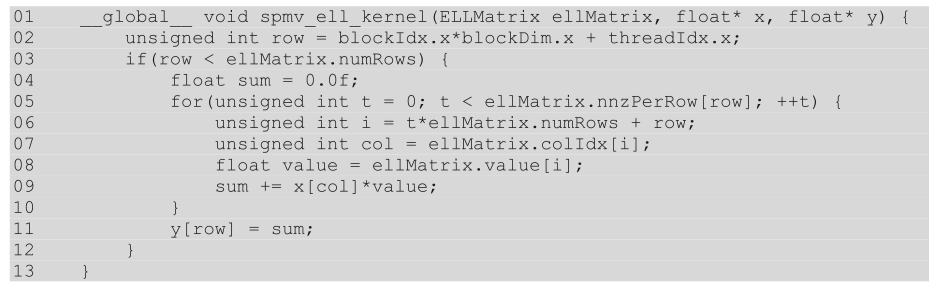
\includegraphics[width=0.9\textwidth]{figs/F14.12.png}
	\caption{\textit{并行 SpMV/ELL 内核。}}
\end{figure}

图 14.11 中我们展示了如何使用的 ELL 格式并行化 SpMV,以及图 14.12 中的并行 SpMV/ELL 内核。 
与 CSR 一样,每个线程都分配给矩阵的不同行(第 02 行),并且边界检查确保该行在边界内(第 03 行)。 
接下来,点积循环遍历每行的非零元素(第 05 行)。 
请注意,SpMV/ELL 内核假设输入矩阵具有一个向量 ellMatrix.nnzPerRow,该向量记录每行中的非零数,
并允许每个线程仅迭代其指定行中的非零数。 
如果输入矩阵没有此向量,则内核可以简单地迭代所有元素(包括填充元素),并且仍然可以正确执行,
因为填充元素的值为零并且不会影响输出值。 接下来,由于压缩矩阵按列优先顺序存储,
因此可以通过将迭代次数 $t$ 乘以行数并加上行索引来找到一维数组中非零元素的索引 $i$ (第 06 行)。 
接下来,线程从 ELL 矩阵数组加载列索引(第 07 行)和非零值(第 08 行)。 
请注意,对这些数组的访问是合并的,因为索引 $i$ 以行表示,而行本身以 threadIdx.x 表示,
这意味着连续的线程具有连续的数组索引。 接下来,线程查找输入值,将其乘以非零值,并将结果累加到局部变量 sum(第 09 行)。 
sum 变量在点积循环开始之前初始化为 0(第 04 行),并在循环结束后累加到输出向量(第 11 行)。

现在我们根据 14.1 节中列出的设计考虑因素来检查 ELL 格式:空间效率、灵活性、可访问性、内存访问效率和负载平衡。 
对于空间效率,我们观察到由于填充元素的空间开销,ELL 格式的空间效率低于 CSR 格式。 
填充元素的开销很大程度上取决于矩阵中非零值的分布。 在一行或少数行具有大量非零元素的情况下,ELL 格式将导致过多的填充元素。 
考虑我们的样本矩阵; 在 ELL 格式中,我们用 $4 \times 3$ 矩阵替换了 $4 \times 4$ 矩阵,并且由于列索引的开销,
我们存储的数据比原始 $4 \times 4$ 矩阵中包含的数据更多。 
举一个更实际的例子,如果 $1000 \times 1000$ 稀疏矩阵有 $1 \%$ 个非零值元素,则平均每行有 10 个非零元素。 
考虑到开销,CSR 表示的大小约为未压缩总大小的 $2 \%$。 假设其中一行有 200 个非零值,而所有其他行的非零值均少于 10 个。
使用 ELL 格式,我们将所有其他行填充到 200 个元素。 这使得 ELL 表示的未压缩总大小约为 $40 \%$,比 CSR 表示大 20 倍。 
当我们从 CSR 格式转换为 ELL 格式时,这就需要一种方法来控制填充元素的数量,我们将在下一节中介绍。 
就灵活性而言,我们观察到在向矩阵添加非零值时,ELL 比 CSR 更灵活。 
在 CSR 中,向行添加非零值需要移位后续行的所有非零值并递增它们的行指针。 
然而,在 ELL 中,只要一行在矩阵中不具有最大数量的非零,就可以通过简单地用实际值替换填充元素来向该行添加非零。

在可访问性方面,ELL 为我们提供了 CSR 和 COO 的可访问性。 
我们在图 14.12 中看到,在给定行索引的情况下,ELL 如何允许我们访问该行的非零值。 
然而,给定非零元素的索引,ELL 还允许我们访问该元素的行索引和列索引。 
列索引很容易找到,因为可以从同一位置 i 的 colIdx 数组访问它。 
然而,由于填充矩阵的规则性质,行索引也可以被访问。 回想一下,非零元素的索引 $i$ 在图 14.9 中计算如下:

\textbf{i = t * ellMatrix.numRows + row}

因此,如果给出 $i$ 并且我们想要查找行,则可以按如下方式找到:

\textbf{row = i \% ellMatrix.numRows}

因为 row 总是小于 ellMatrix.numRows,所以 row\%ellMatrix.numRows 只是 row 本身。 
ELL 的这种可访问性允许跨行以及非零元素并行化。

对于内存访问效率,我们参考图 14.11 中的物理视图,了解线程在点积循环的第一次迭代期间如何从内存访问矩阵数据。 
访问模式使得连续的线程访问连续的数据元素。 
通过按列优先顺序排列元素,所有相邻线程现在都可以访问相邻内存位置,从而实现内存合并,从而更有效地利用内存带宽。 
一些 GPU 架构,尤其是老一代的 GPU 架构,对于内存合并有更严格的地址对齐规则。 
通过在转置之前向矩阵末尾添加几行,可以强制 SpMV/ELL 内核的每次迭代完全对齐到架构上指定的对齐单元(例如 64 字节)。

对于负载平衡,我们观察到 SpMV/ELL 仍然表现出与 SpMV/CSR 相同的负载不平衡,因为每个线程仍然循环遍历其负责的行中的非零数。 
因此ELL并没有解决控制发散的问题。

总之,ELL 格式在 CSR 格式的基础上进行了改进,它允许更灵活地通过替换填充元素来添加非零值、更好的可访问性,
以及最重要的是,在 SpMV/ELL 中提供更多内存合并机会。 
然而,ELL的空间效率比CSR差,并且SpMV/ELL的控制散度与SpMV/CSR一样差。 
在下一节中,我们将了解如何改进 ELL 格式以解决空间效率和控制发散问题。

\subsection{使用混合 ELL-COO 格式调节填充}
当一行或少量行具有大量非零元素时,ELL 格式中的低空间效率和控制发散问题最为明显。 
如果我们有一种机制从这些行中“拿走”一些元素,我们就可以减少 ELL 中填充元素的数量,并减少控制发散。 
答案在于 $\mathrm{COO}$ 格式的一个重要用例。

COO 格式可用于限制 ELL 格式中的行长度。 
在将稀疏矩阵转换为 ELL 之前,我们可以从具有大量非零元素的行中取出一些元素,并将这些元素放入单独的 COO 存储中。 
我们可以对其余元素使用 SpMV/ELL。 通过从超长行中删除多余的元素,可以显着减少其他行的填充元素的数量。 
然后我们可以使用 SpMV/COO 来完成工作。 这种采用两种格式协作完成计算的方法通常称为混合方法。

\begin{figure}[H]
	\centering
	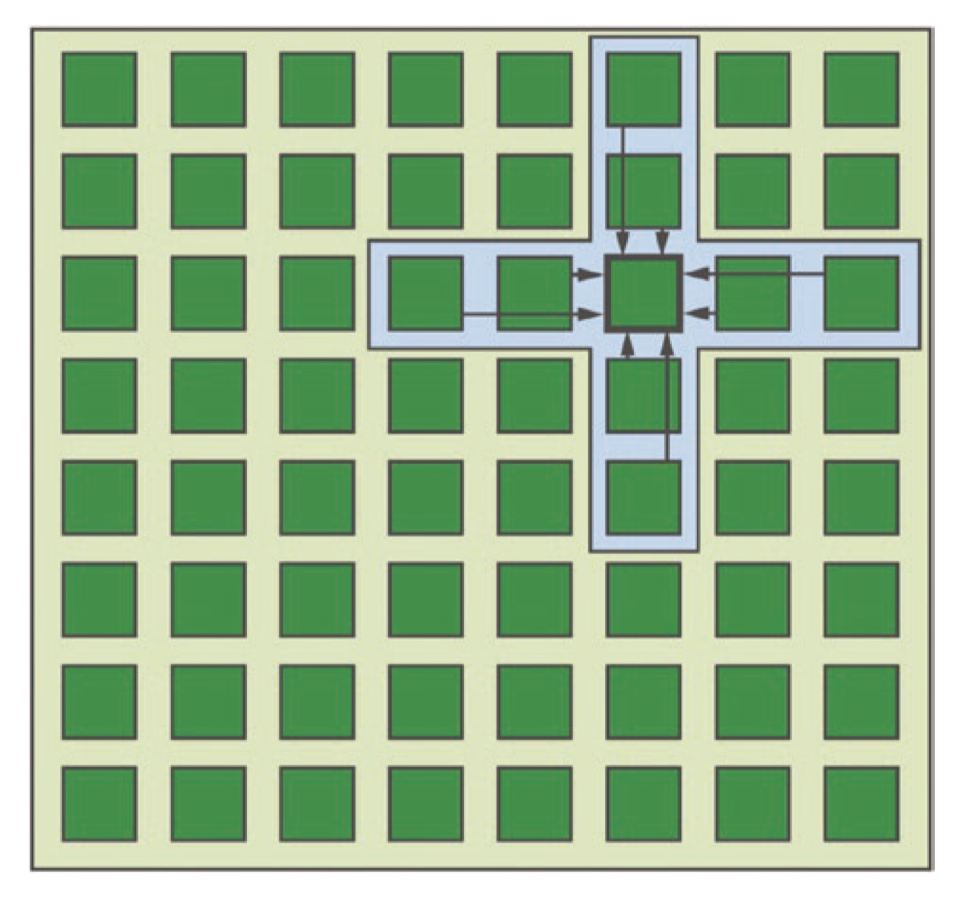
\includegraphics[width=0.9\textwidth]{figs/F14.3.png}
	\caption{\textit{混合 ELL-COO 示例。}}
\end{figure}

图 14.13 说明了如何使用混合 ELL-COO 格式表示示例矩阵。 
我们看到,仅在 ELL 格式中,第 1 行和第 6 行的非零元素数量最多,导致其他行填充过多。 
为了解决这个问题,我们从 ELL 表示中删除第 2 行的最后三个非零元素和第 6 行的最后两个非零元素,
并将它们移动到单独的 $\mathrm{COO}$ 表示中。 
通过删除这些元素,我们将小型稀疏矩阵中所有行中非零元素的最大数量从 5 减少到 2 。 
如图 14.13 所示,我们将填充元素的数量从 22 个减少到 3 个。更重要的是,所有线程现在只需要进行两次迭代。

读者可能想知道,将 COO 元素与 ELL 格式分离的额外工作是否会产生过多的开销。 答案是,这取决于情况。 
在稀疏矩阵仅用于一次 SpMV 计算的情况下,这项额外工作确实会产生大量开销。 
然而,在许多实际应用中,SpMV 在迭代求解器中重复地在同一稀疏核上执行。 
在求解器的每次迭代中,$\mathrm{x}$和$\mathrm{y}$向量发生变化,但稀疏矩阵保持不变,
因为其元素对应于正在求解的线性方程组的系数,并且 这些系数在迭代之间不会改变。 
因此,为生成混合 ELL 和 COO 表示所做的工作可以在多次迭代中分摊。 我们将在下一节中回到这一点。

现在我们根据第 14.1 节中列出的设计考虑因素来检查混合 ELL-COO 格式:空间效率、灵活性、可访问性、内存访问效率和负载平衡。 
对于空间效率,我们观察到混合 ELL-COO 格式比单独的 ELL 格式具有更好的空间效率,因为它减少了所使用的填充量。

为了灵活性,我们观察到在向矩阵添加非零值时,混合 ELL-COO 格式比仅 ELL 更灵活。 
使用 ELL,我们可以通过替换包含非零元素的行的填充元素来添加非零元素。 
使用混合 COO-ELL,我们还可以通过替换填充元素来添加非零值。 
但是,如果该行没有任何可以在 ELL 部分中替换的填充元素,我们也可以将非零附加到格式的 COO 部分。

对于可访问性,我们观察到与单独的 ELL 格式相比,混合 ELL-COO 格式牺牲了可访问性。 
特别是,在给定行索引的情况下,并不总是可以访问该行中的所有非零值。 只能对符合格式的 ELL 部分的行进行此类访问。 
如果该行溢出到 $\mathrm{COO}$ 部分,则查找该行的所有非零值将需要搜索 $\mathrm{COO}$ 部分,这是昂贵的。

为了提高内存访问效率,SpMV/ELL 和 SpMV/COO 都表现出对稀疏矩阵的合并内存访问。 
因此,它们的组合也将导致合并访问模式。

为了实现负载平衡,从格式的 ELL 部分中的长行中删除非零可以减少 SpMV/ELL 内核的控制分歧。 
这些非零值被放置在格式的 $\mathrm{COO}$ 部分,这不会影响控制发散,因为正如我们所见,SpMV/COO 不表现出控制发散。

总之,与单独的 ELL 格式相比,混合 ELL-COO 格式通过减少填充提高了空间效率,为向矩阵添加非零提供了更大的灵活性,
保留了合并的内存访问模式,并减少了控制发散。 
付出的代价是可访问性的一个小限制,如果给定行溢出到格式的 $\mathrm{COO}$ 部分,则访问该行的所有非零值将变得更加困难。

\subsection{使用 JDS 格式减少控制发散}
我们已经看到,在访问 SpMV 中的稀疏矩阵时,可以使用 ELL 格式来实现合并内存访问模式,
并且混合 ELL-COO 格式可以通过减少填充进一步提高空间效率,还可以减少控制发散。 
在本节中,我们将研究另一种格式,它可以在 SpMV 中实现合并内存访问模式,并且无需执行任何填充即可减少控制发散。 
这个想法是根据行的长度对行进行排序,例如从最长到最短。 
由于排序矩阵看起来很像三角矩阵,因此该格式通常称为锯齿状对角存储 (JDS) 格式。

\begin{figure}[H]
	\centering
	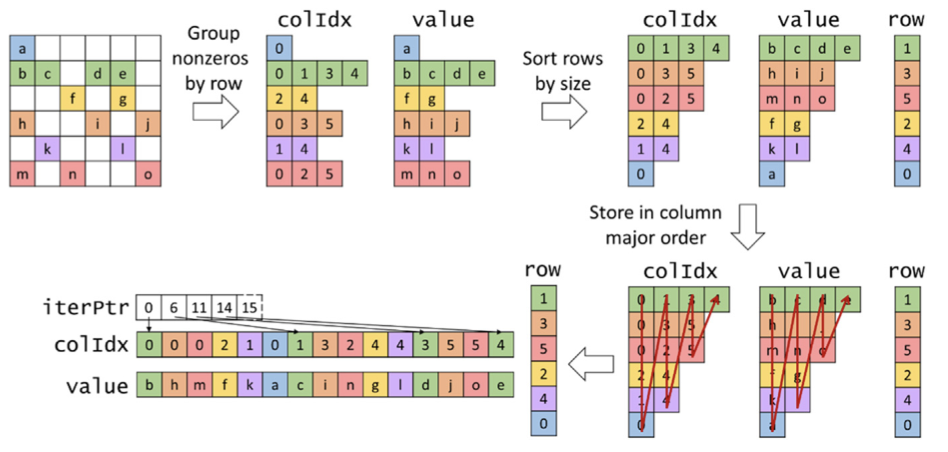
\includegraphics[width=0.9\textwidth]{figs/F14.14.png}
	\caption{\textit{JDS 存储格式示例。}}
\end{figure}

图 14.14 说明了如何使用 JDS 格式存储矩阵。 首先,非零值按行分组,如 CSR 和 ELL 格式所示。 
接下来,按每行中非零的数量按升序对行进行排序。 当我们对行进行排序时,我们通常会维护一个附加的行数组来保留原始行的索引。 
每当我们在排序过程中交换两行时,我们也会交换行数组中相应的元素。 因此我们可以始终跟踪所有行的原始位置。 
对行进行排序后,值数组中的非零值及其在 colIdx 数组中相应的列索引将按列优先顺序存储。 
添加 iterPtr 数组来跟踪每次迭代的非零元素的开头。

\begin{figure}[H]
	\centering
	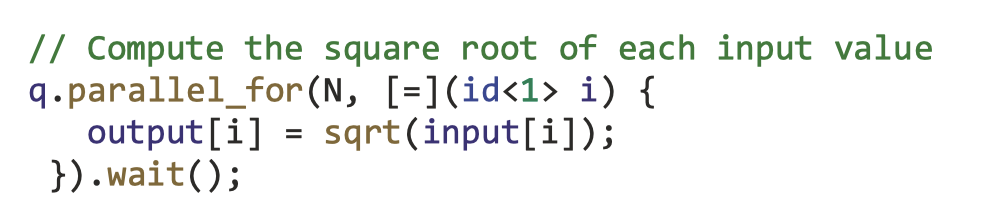
\includegraphics[width=0.9\textwidth]{figs/F14.15.png}
	\caption{\textit{SpMV 与 JDS 格式并行化的示例。}}
\end{figure}

图 14.15 说明了如何使用 JDS 格式并行化 SpMV。 每个线程被分配给矩阵的一行,并迭代该行的非零值,一路执行点积。 
线程使用 iterPtr 数组来标识每次迭代的非零值开始的位置。 
从图 14.15 右侧的物理视图(描述每个线程的第一次迭代)中应该可以清楚地看出,
线程以合并的方式访问 JDS 数组中的非零值和列索引。 实现 SpMV/JDS 的代码留作练习。

在 JDS 格式的另一种变体中,行在排序后可以分为行段。 
由于行已排序,因此节中的所有行可能具有或多或少统一数量的非零元素。 然后我们可以生成每个部分的 ELL 表示。 
在每个部分中,我们只需要填充行以使该行与该部分中的最大元素数相匹配。 
与整个矩阵的一个 ELL 表示相比,这将大大减少填充元素的数量。 在 JDS 的这个变体中,不需要 iterPtr 数组。 
相反,我们需要一个仅指向每个 ELL 部分开头的部分指针数组(而不是每次迭代)。

读者应该问,对行进行排序是否会导致线性方程组的解不正确。 回想一下,我们可以自由地重新排序线性系统的方程而不改变解。 
只要我们对 y 元素和行进行重新排序,我们就有效地对方程进行了重新排序。 因此我们最终会得到正确的解决方案。 
唯一的额外步骤是使用行数组将最终解决方案重新排序回原始顺序。 另一个问题是排序是否会产生大量开销。 
答案与我们在混合 ELL-COO 方法中看到的类似。 
只要在迭代求解器中使用 SpMV/JDS 内核,就可以执行此类排序以及最终解决方案 $x$ 元素的重新排序,
并在求解器的多次迭代中分摊成本。

现在我们根据 14.1 节中列出的设计考虑因素来检查 ELL 格式:空间效率、灵活性、可访问性、内存访问效率和负载平衡。 
就空间效率而言,JDS 格式比 ELL 格式更节省空间,因为它避免了填充。 
每个部分使用 ELL 的 JDS 变体都有填充,但填充量比 ELL 格式少。

为了灵活性,JDS 格式并不容易将非零添加到矩阵的一行。 
它甚至比 CSR 格式更不灵活,因为添加非零会改变行的大小,这可能需要对行进行重新排序。

对于可访问性,JDS 格式类似于 CSR 格式,因为它允许我们在给定行索引的情况下访问该行的非零元素。 
另一方面,它并不像 COO 和 ELL 格式那样,在给定非零值的情况下轻松访问该非零值的行索引和列索引。 
就内存访问效率而言,JDS 格式类似于 ELL 格式,因为它按列优先顺序存储非零值。 
因此,JDS 格式使得对稀疏矩阵的访问能够以合并的方式发生。 
由于 JDS 不需要填充,因此每次迭代中内存访问的起始位置(如图 14.15 的物理视图所示)可以以任意方式变化。 
因此,没有简单、廉价的方法来强制 SpMV/JDS 内核的所有迭代从体系结构指定的对齐边界开始。 
由于缺乏强制对齐的选项,JDS 的内存访问效率低于 ELL 中的内存访问。

对于负载平衡,JDS 的独特功能是它对矩阵的行进行排序,以便同一warp中的线程可能会迭代相似长度的行。 
因此JDS对于减少控制发散是有效的。

\subsection{总结}
在本章中,我们将稀疏矩阵计算作为一种重要的并行模式提出。 稀疏矩阵在许多涉及复杂现象建模的现实应用中非常重要。 
此外,稀疏矩阵计算是许多大型实际应用程序依赖于数据的性能行为的一个简单示例。 
由于零元素数量较多,因此使用压缩技术来减少对这些零元素执行的存储量、内存访问量和计算量。 
使用这种模式,我们引入了使用混合方法和排序/分区的正则化概念。 这些正则化方法用于许多实际应用中。 
有趣的是,一些正则化技术将零元素重新引入到压缩表示中。 我们使用混合方法来减轻可能引入过多零元素的病态情况。 
读者可以参考 Bell 和 Garland (2009),并鼓励读者尝试不同的稀疏数据集,
以更深入地了解本章介绍的各种 SpMV 内核的数据依赖性能行为。

应该清楚的是,并行 SpMV 内核的执行效率和内存带宽效率都取决于输入数据矩阵的分布。 
这与我们迄今为止研究的大多数内核有很大不同。 然而,这种依赖于数据的性能行为在实际应用中非常常见。 
这就是并行 SpMV 如此重要的并行模式的原因之一。 它很简单,但它说明了许多复杂并行应用程序中的重要行为。

与稠密矩阵计算相比,我们想对稀疏矩阵计算的性能进行补充说明。 
一般来说,稀疏矩阵计算通过 CPU 或 GPU 实现的 FLOPS 等级比密集矩阵计算低得多。 
对于 SpMV 来说尤其如此,其中稀疏矩阵中没有数据重用。 OP/B 基本上为 0.25,将可实现的 FLOPS 率限制为峰值性能的一小部分。 
各种格式对于 CPU 和 GPU 都很重要,因为两者在执行 SpMV 时都受到内存带宽的限制。 
过去,人们常常对 CPU 和 GPU 上此类计算的低 FLOPS 评级感到惊讶。 读完这一章,你应该不再感到惊讶了。